	\section{Цель работы}
		Разработать экспертную систему на основе Байесовской сети доверия с использованием среды HUGIN.
		
	\section{Предметная область}
		Целевая ЭС выполняет функцию оценки платформ для социальной торговли. Социальная торговля -- онлайн-трейдинг на финансовых рынках в рамках социальной платформы, внутри которой трейдеры взаимодействуют друг с другом.
		
		На рисунке \ref{tree} изображено дерево целей экспертной системы. 
		
		\begin{figure}[ht] 
			\center
			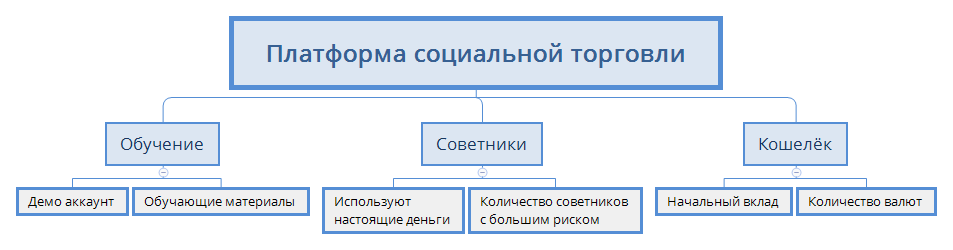
\includegraphics [width=\textwidth] {social-trading}
			\caption{Дерево целей} 
			\label{tree}
		\end{figure}
		\FloatBarrier
		
		На рисунке \ref{bn} представлена проектируемая Байесовская сеть доверия, составленная на основе дерева целей.
		
		\begin{figure}[ht] 
			\center
			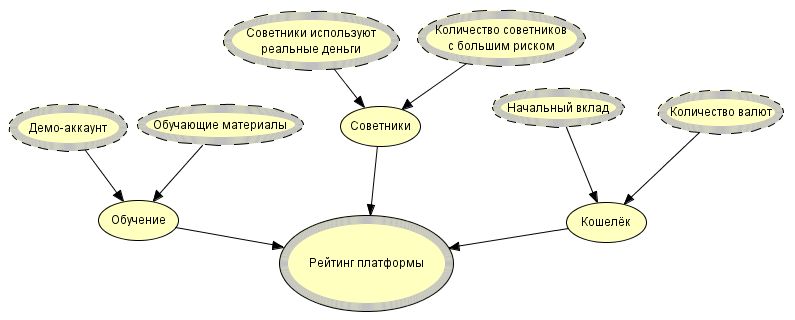
\includegraphics [width=0.8\textwidth] {bayes-tree}
			\caption{Байесовская сеть доверия} 
			\label{bn}
		\end{figure}
		\FloatBarrier
		
	\section{Таблицы условных вероятностей}
	
		Далее представлены таблицы условных вероятностей для каждой вершины БСД. На рисунке \ref{input} представлены 
		таблицы вероятностей вершин, отмеченных как входные.
		
		\begin{figure}[ht]
			\begin{minipage}[ht]{0.49\linewidth}
				\center{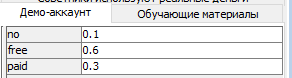
\includegraphics[width=0.8\linewidth]{demo} \\ а) Демо-аккаунт}
			\end{minipage}
			\hfill
			\begin{minipage}[ht]{0.49\linewidth}
				\center{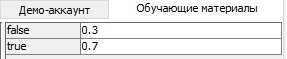
\includegraphics[width=0.8\linewidth]{materials} \\ б) Обучающие материалы}
			\end{minipage}
			\vfill
			\begin{minipage}[ht]{0.49\linewidth}
				\center{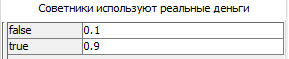
\includegraphics[width=0.8\linewidth]{real-money} \\ в) Советники используют реальные деньги}
			\end{minipage}
			\hfill
			\begin{minipage}[ht]{0.49\linewidth}
				\center{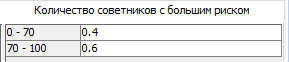
\includegraphics[width=0.8\linewidth]{risk} \\ г) Количество советников с большим риском}
			\end{minipage}
			\vfill
			\begin{minipage}[ht]{0.49\linewidth}
				\center{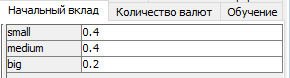
\includegraphics[width=0.8\linewidth]{investment} \\ д) Начальный вклад}
			\end{minipage}
			\hfill
			\begin{minipage}[ht]{0.49\linewidth}
				\center{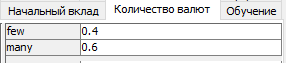
\includegraphics[width=0.8\linewidth]{currencies} \\ е) Количество валют}
			\end{minipage}
			\caption{Таблицы условных вероятностей для входных вершин.}
			\label{input}  
		\end{figure}
	
		На рисунке \ref{output} представлены 
		таблицы вероятностей остальных вершин.
		
		\begin{figure}[ht]
			\begin{minipage}[ht]{0.49\linewidth}
				\center{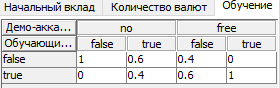
\includegraphics[width=0.8\linewidth]{education} \\ а) Обучение}
			\end{minipage}
			\hfill
			\begin{minipage}[ht]{0.49\linewidth}
				\center{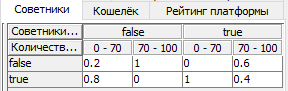
\includegraphics[width=0.8\linewidth]{advisers} \\ б) Советники}
			\end{minipage}
			\vfill
			\center{
				\begin{minipage}[ht]{0.49\linewidth}
					\center{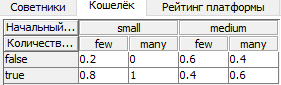
\includegraphics[width=0.8\linewidth]{wallet} \\ в) Кошелёк}
				\end{minipage}
			}
			\vfill
			\begin{minipage}[ht]{0.8\linewidth}
				\center{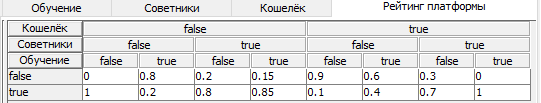
\includegraphics[width=0.8\linewidth]{rating} \\ д) Рейтинг платформы}
			\end{minipage}
			\caption{Таблицы условных вероятностей для остальных вершин.}
			\label{output}  
		\end{figure}
		\FloatBarrier
	\newpage
	\section{Примеры выполнения}
	
	На рисунке \ref{examples} изображены примеры работы БСД.
	\begin{figure}[ht]
		\begin{minipage}[ht]{0.49\linewidth}
			\center{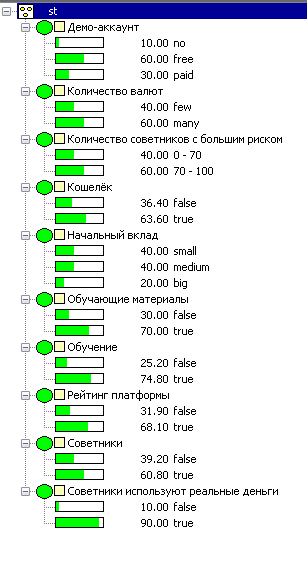
\includegraphics[width=0.8\linewidth]{result-normal} \\ а) Пример хорошей платформы}
		\end{minipage}
		\hfill
		\begin{minipage}[ht]{0.49\linewidth}
			\center{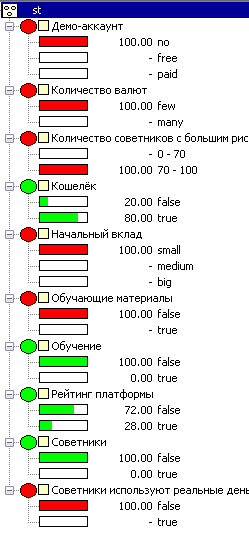
\includegraphics[width=0.85\linewidth]{result-bad} \\ б) Пример плохой платформы}
		\end{minipage}
		\caption{Примеры выполнения.}
		\label{examples}  
	\end{figure}

	
	\section{Вывод}
		В результате данной работы была спроектирована разработана ЭС на основе Байесовской сети доверия, которая позволяет дать экспертную оценку платформам социальной торговли по введенным параметрам. Изучена программа HUGIN.